\documentclass[11pt]{article}

\usepackage[T1]{fontenc}
\usepackage{lmodern}
\usepackage{microtype}
\usepackage[margin=1in]{geometry}
\usepackage{amsmath,amssymb,amsthm,mathtools}
\usepackage{graphicx}
\usepackage{xcolor}
\usepackage{enumitem}
\usepackage{booktabs}
\usepackage{fancyhdr}
\usepackage[hidelinks]{hyperref}

\definecolor{accent}{HTML}{174A6E}
\definecolor{statusbg}{HTML}{EEF5F8}
\definecolor{statusline}{HTML}{6B95AD}

\newtheorem{theorem}{Theorem}
\newtheorem{lemma}[theorem]{Lemma}
\newtheorem{corollary}[theorem]{Corollary}
\theoremstyle{definition}
\newtheorem{definition}[theorem]{Definition}
\theoremstyle{remark}
\newtheorem{remark}[theorem]{Remark}

\newcommand{\E}{\mathbb E}
\newcommand{\Pp}{\mathbb P}
\newcommand{\asympc}{\mathrel{\asymp}}
\newcommand{\lesssimc}{\mathrel{\lesssim}}
\newcommand{\gtrsimc}{\mathrel{\gtrsim}}

\pagestyle{fancy}
\fancyhf{}
\fancyhead[L]{\small\textcolor{accent}{Lacunary endpoint generators}}
\fancyhead[R]{\small arXiv:2407.14870}
\fancyfoot[C]{\thepage}
\setlength{\headheight}{14pt}

\title{Lacunary Endpoint Generators:\\
Nonuniqueness at Both Orlicz Boundaries}
\author{Candidate counterexample packet for human verification\\
\small Run \texttt{fa\_banach\_001}, lane 17, model GPT5.6}
\date{11 August 2026}

\begin{document}
\maketitle

\noindent
\colorbox{statusbg}{%
  \parbox{0.965\textwidth}{%
    \textcolor{statusline}{\rule{2pt}{1.15em}}\hspace{0.6em}
    \textbf{Status: candidate counterexample, likely valid.}
    The packet gives explicit non-quasi-equivalent generators at both endpoint
    scales.  At the quadratic logarithmic endpoint it contradicts Theorem~4.2
    of Braverman (1993) as printed and the uniqueness conclusion repeated in
    Remark~5.1 of Astashkin's 2024 survey.  Expert review is required before
    any public novelty claim.
  }%
}

\begin{abstract}
Fix $1\leq p<2$.  For a broad class of increasing functions $W$, we construct
two pairs of symmetric $L_p$ random variables.  The two members of each pair
have non-quasi-equivalent tails, but their independent copies span the same
Orlicz sequence space in $L_p$.  The two Orlicz functions have endpoint
asymptotics
\[
  M_-(t)\asymp \frac{t^p}{W(\log(1/t))},
  \qquad
  M_+(t)\asymp t^2W(\log(1/t)).
\]
In particular this proves nonuniqueness for
$t^p/\log^\alpha(e/t)$ and $t^2\log^\alpha(e/t)$ for every
$\alpha>0$.  Taking $W(s)=s$ in the upper construction gives a generator of
$\ell_{t^2\log(e/t)}$ whose lacunary tail is not comparable with $x^{-2}$.
This is a direct counterexample to the quadratic-boundary implication in the
cited 1993 theorem.
\end{abstract}

\section{Source question and the published endpoint claim}

The source target is S.~V.~Astashkin, \emph{On subspaces of Orlicz spaces
spanned by independent copies of a mean zero function}, arXiv:2407.14870
\cite{Ast24a}.  On source PDF page~3 it recalls the following natural
question.

\begin{figure}[ht]
  \centering
  
\includegraphics[width=\textwidth]{figures/open_problem_crop.png}
  \caption{The source paper's uniqueness question and its statement that only
  partial answers were known, rendered from source PDF page~3.}
  \label{fig:source-question}
\end{figure}

\paragraph{Transcription.}
If $1\leq p<2$ and a mean-zero $f\in L_p$ has independent copies spanning
the canonical basis of an Orlicz sequence space $\ell_\psi$, is the
distribution of $f$ uniquely determined, up to equivalence for large values
of the argument, by $\psi$?  The source notes that only partial solutions are
known.

Astashkin's survey \cite[Remark~5.1]{Ast24survey} states, by reference to
Braverman's Theorem~4.2 \cite{Br93}, that the distribution is unique for
\[
  \psi(t)=t^2\log_2(2/t).
\]
The precise theorem in the cited paper is reproduced in
Figure~\ref{fig:braverman}.  With $h(x)$ slowly varying and
\[
  \Psi_2(t)=t^2\int_0^{1/t}\frac{h(y)}{y}\,dy,
\]
it claims equivalence between the two-sided coefficient estimate for
$\ell_{\Psi_2}$ and the pointwise tail estimate
$\Pp\{|X|\geq x\}\asymp x^{-2}h(x)$.  One may take $h=1$ for large $x$ and
modify it near zero; then $\Psi_2(t)\asymp t^2\log(e/t)$.

\begin{figure}[ht]
  \centering
  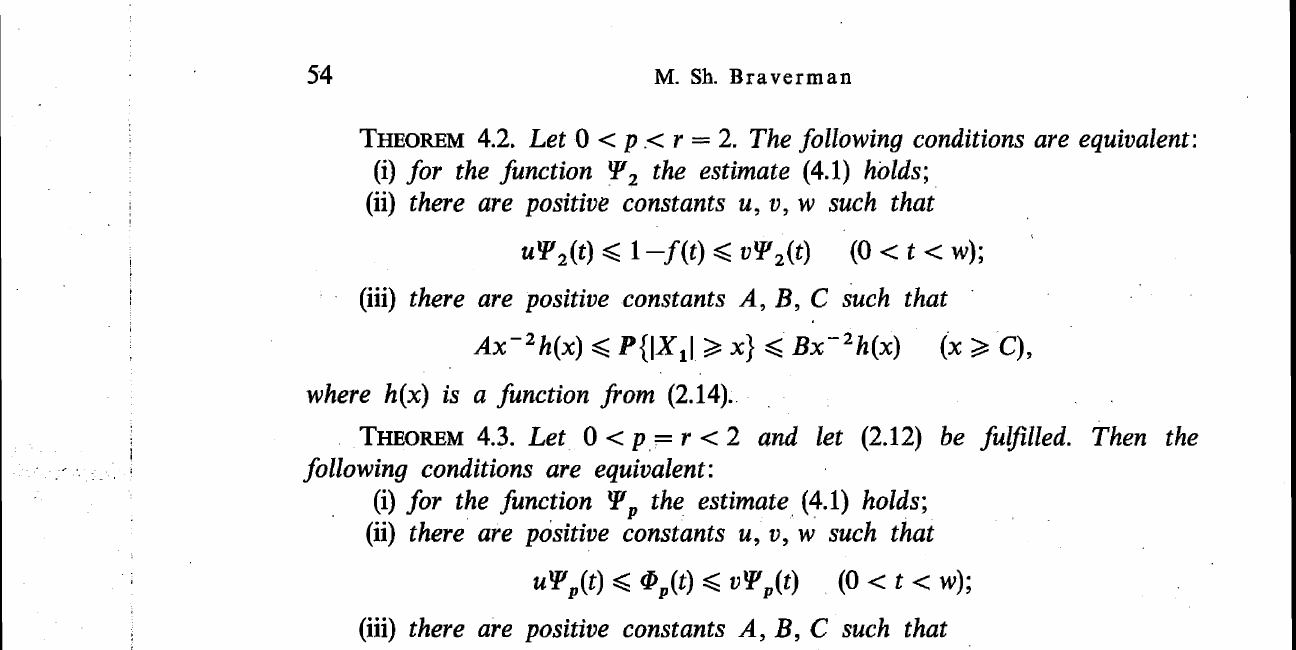
\includegraphics[width=\textwidth]{figures/braverman_theorem_4_2_crop.png}
  \caption{Braverman's Theorem~4.2, journal page~54 (physical PDF page~10).}
  \label{fig:braverman}
\end{figure}

\section{Definitions and the disjointification reduction}

For a random variable $Z$, write
\[
  n_Z(\tau):=\Pp\{|Z|>\tau\},\qquad \tau>0.
\]
The robust failure of quasi-equivalence used below is
\begin{equation}\label{eq:robust-failure}
  \text{for every }C\geq1,\qquad
  \limsup_{\tau\to\infty}\frac{n_X(C\tau)}{n_Y(\tau)}=\infty.
\end{equation}
This is exactly the separation condition used in the known lower-endpoint
example \cite[Theorem~5.3]{Ast24survey}.

Put
\begin{equation}\label{eq:Np}
  N_p(u):=
  \begin{cases}
    u^2,&0\leq u\leq1,\\
    \dfrac2p u^p+1-\dfrac2p,&u\geq1.
  \end{cases}
\end{equation}
This is an Orlicz function and
$N_p(u)\asymp\min\{u^p,u^2\}$.  Thus the function Orlicz space
$L_{N_p}(0,\infty)$ is $L_p+L_2$ up to equivalence of norms.  For a positive
random variable $Z$, define
\begin{equation}\label{eq:modular}
  M_Z(t):=\E N_p(tZ).
\end{equation}
Disjoint copies of $Z$ in $L_{N_p}(0,\infty)$ span $\ell_{M_Z}$ exactly in
Luxemburg modulars.  The Johnson--Schechtman/Rosenthal disjointification
estimate \cite{JS89}, in the form recorded in the source literature
\cite[\S\,2.4]{Ast24a}, implies that if $f=\varepsilon Z$, where
$\varepsilon$ is an independent Rademacher sign, then independent copies of
$f$ in $L_p(0,1)$ are equivalent to the canonical basis of $\ell_{M_Z}$.
Consequently it is enough to construct positive $X,Y\in L_p$ such that
$M_X\asymp M_Y$ near zero and \eqref{eq:robust-failure} holds.

Notice also that $M_Z$ is $p$-convex and $2$-concave: after the substitutions
$t=u^{1/p}$ and $t=u^{1/2}$, these properties hold termwise for
$N_p(tZ)$ and are preserved by integration.

\section{Proof intuition}

The modular \eqref{eq:modular} smooths a distribution across the threshold
$Z=1/t$.  At the lower endpoint, its main term is the $p$-moment of the tail;
at the upper endpoint, it is the truncated second moment below the threshold.
Pointwise tail data can therefore be moved between extremely distant atoms
without changing the smoothed modular by more than a constant.

We put atoms at heights $A_k=\exp(2^k)$.  One distribution uses every height,
whereas the other uses only odd-indexed heights.  Since adjacent logarithmic
scales differ only by a factor two (or four on the odd grid), both modulars
remain comparable.  In the enormous gap between $A_{2j+1}$ and $A_{2j+2}$,
however, the full distribution still sees its $A_{2j+2}$ atom while the odd
distribution must wait until $A_{2j+3}$.  The resulting tail ratio grows
doubly exponentially and defeats every fixed rescaling.

\section{The geometrically doubling construction}

\begin{theorem}[Two endpoint nonuniqueness families]\label{thm:main}
Let $1\leq p<2$.  Suppose $W:[2,\infty)\to(0,\infty)$ is nondecreasing and
there are constants $1<\lambda\leq\Lambda<\infty$ such that
\begin{equation}\label{eq:W-doubling}
  \lambda\leq\frac{W(2s)}{W(s)}\leq\Lambda,
  \qquad s\geq2.
\end{equation}
Then there are symmetric mean-zero random variables
$f_-,g_-,f_+,g_+\in L_p(0,1)$ with the following properties.
\begin{enumerate}[label=\textup{(\roman*)}]
  \item The independent copies of $f_-$ and $g_-$ are both equivalent in
  $L_p$ to the canonical basis of the same Orlicz sequence space
  $\ell_{M_-}$, where
  \[
    M_-(t)\asymp \frac{t^p}{W(\log(1/t))}\qquad(t\downarrow0).
  \]
  \item The independent copies of $f_+$ and $g_+$ are both equivalent in
  $L_p$ to the canonical basis of the same Orlicz sequence space
  $\ell_{M_+}$, where
  \[
    M_+(t)\asymp t^2W(\log(1/t))\qquad(t\downarrow0).
  \]
  \item Each pair has non-quasi-equivalent distributions in the strong sense
  of \eqref{eq:robust-failure}.
\end{enumerate}
The same conclusion holds when \eqref{eq:W-doubling} is imposed only for all
sufficiently large $s$.
\end{theorem}

\begin{proof}
Set
\[
  u_k:=2^k,\qquad A_k:=e^{u_k},\qquad w_k:=W(u_k),\qquad k\geq1.
\]
Choose positive normalizing constants so that the following masses sum to at
most one, and put all unused probability at zero.  Define positive random
variables $X_-,Y_-,X_+,Y_+$ by
\begin{alignat}{3}
  \Pp\{X_-=A_k\}&=c_-w_k^{-1}A_k^{-p},&\qquad& k\geq1,
  &\qquad \Pp\{Y_-=A_k\}&=d_-w_k^{-1}A_k^{-p},\quad k\text{ odd},
  \label{eq:lower-masses}\\
  \Pp\{X_+=A_k\}&=c_+w_kA_k^{-2},&& k\geq1,
  &\Pp\{Y_+=A_k\}&=d_+w_kA_k^{-2},\quad k\text{ odd}.
  \label{eq:upper-masses}
\end{alignat}
Condition \eqref{eq:W-doubling} gives $w_{k+1}/w_k\in[\lambda,\Lambda]$.
Therefore
\[
  \E X_-^p=c_-\sum_{k\geq1}w_k^{-1}<\infty,
  \qquad
  \E X_+^p=c_+\sum_{k\geq1}w_ke^{-(2-p)u_k}<\infty,
\]
and the same holds for the odd-grid variables.  Thus all four are in $L_p$.

We first estimate the full-grid modulars.  Let $s=\log(1/t)$ and choose $m$
so that $u_m\leq s<u_{m+1}$.  Since $N_p(v)\asymp\min(v^p,v^2)$,
\begin{align}
  M_{X_-}(t)
  &\asympc
  t^2\sum_{k\leq m}w_k^{-1}e^{(2-p)u_k}
  +t^p\sum_{k>m}w_k^{-1},\label{eq:lower-split}\\
  M_{X_+}(t)
  &\asympc
  t^2\sum_{k\leq m}w_k
  +t^p\sum_{k>m}w_ke^{-(2-p)u_k}.
  \label{eq:upper-split}
\end{align}

For the lower modular, the second sum is a geometric tail and
\begin{equation}\label{eq:lower-tail}
  \sum_{k>m}w_k^{-1}\asympc w_{m+1}^{-1}\asympc W(s)^{-1}.
\end{equation}
The summands $w_k^{-1}e^{(2-p)u_k}$ in the first sum are eventually increasing
by a factor at least two, because $u_{k+1}-u_k=u_k$ and the exponential
dominates the fixed factor $w_{k+1}/w_k$.  Finitely many initial indices can
be absorbed into the constant, so
\[
  \sum_{k\leq m}w_k^{-1}e^{(2-p)u_k}\lesssimc
  w_m^{-1}e^{(2-p)u_m}.
\]
Using $W(s)/w_m\leq\Lambda$ and $s\geq u_m$, the ratio of the resulting first
term in \eqref{eq:lower-split} to $t^p/W(s)$ is at most
\[
  \frac{W(s)}{w_m}e^{-(2-p)(s-u_m)}\leq\Lambda.
\]
Together with \eqref{eq:lower-tail}, this proves
\begin{equation}\label{eq:lower-result}
  M_{X_-}(t)\asympc \frac{t^p}{W(s)}.
\end{equation}

For the upper modular, geometric growth gives
\begin{equation}\label{eq:upper-head}
  \sum_{k\leq m}w_k\asympc w_m\asympc W(s),
\end{equation}
which already supplies both bounds at the target scale.  The terms
$w_ke^{-(2-p)u_k}$ are eventually decreasing by a factor at least two, so the
tail in \eqref{eq:upper-split} is dominated by its first term.  Since
$w_{m+1}/W(s)\leq\Lambda$ and $s<u_{m+1}$,
\[
  \frac{t^p w_{m+1}e^{-(2-p)u_{m+1}}}{t^2W(s)}
  =\frac{w_{m+1}}{W(s)}e^{-(2-p)(u_{m+1}-s)}
  \leq\Lambda.
\]
Consequently
\begin{equation}\label{eq:upper-result}
  M_{X_+}(t)\asympc t^2W(s).
\end{equation}

The identical proof applies on the odd grid.  Indeed its logarithmic scales
are $u_{2j+1}=2\cdot4^j$, consecutive scales have ratio four, and
\[
  \lambda^2\leq \frac{W(4s)}{W(s)}\leq\Lambda^2.
\]
For $s$ between two consecutive odd scales, monotonicity and the last display
make $W(s)$ comparable with the preceding odd-grid weight.  Hence
\begin{equation}\label{eq:both-grids}
  M_{Y_-}(t)\asympc M_{X_-}(t),
  \qquad M_{Y_+}(t)\asympc M_{X_+}(t).
\end{equation}

It remains to prove robust tail separation.  Fix $C\geq1$.  For all large
$j$, the gap $A_{2j+2}/A_{2j+1}$ exceeds $2C$; choose
\[
  \tau_j:=\frac{A_{2j+2}}{2C}.
\]
Then both $\tau_j$ and $C\tau_j$ lie strictly between $A_{2j+1}$ and
$A_{2j+2}$.  The full-grid tail at $C\tau_j$ contains its $A_{2j+2}$ atom,
whereas the first atom in the odd-grid tail at $\tau_j$ is $A_{2j+3}$.
The rest of the odd tail is at most a fixed multiple of that first atom,
again because the double exponential dominates the geometric variation of
$w_k$.  For the lower pair the ratio of the decisive masses is bounded below
by a fixed positive multiple of
\[
  \frac{w_{2j+3}}{w_{2j+2}}
  e^{p(u_{2j+3}-u_{2j+2})}
  \geq \lambda e^{p u_{2j+2}}\longrightarrow\infty,
\]
and for the upper pair it is bounded below by a fixed positive multiple of
\[
  \frac{w_{2j+2}}{w_{2j+3}}
  e^{2(u_{2j+3}-u_{2j+2})}
  \geq \Lambda^{-1}e^{2u_{2j+2}}\longrightarrow\infty.
\]
This proves \eqref{eq:robust-failure} for both pairs.

Finally take independent Rademacher signs and set
$f_-=\varepsilon X_-$, $g_-=\varepsilon Y_-$,
$f_+=\varepsilon X_+$, and $g_+=\varepsilon Y_+$.  They are symmetric,
mean zero, and in $L_p$.  The disjointification reduction preceding the
theorem, together with \eqref{eq:both-grids}, proves the asserted equivalence
of their independent-copy sequences.  If \eqref{eq:W-doubling} holds only
eventually, discard finitely many initial atoms; this changes none of the
asymptotic conclusions.
\end{proof}

\begin{corollary}[Logarithmic and log--log endpoints]\label{cor:logs}
For every $1\leq p<2$, $\alpha>0$, and $\beta\in\mathbb R$, there are two
non-quasi-equivalent generators for each of the Orlicz sequence spaces with
small-argument asymptotics
\[
  \frac{t^p}
  {\log^\alpha(e/t)\,[\log\log(e^e/t)]^\beta}
  \quad\text{and}\quad
  t^2\log^\alpha(e/t)\,[\log\log(e^e/t)]^\beta.
\]
In particular one may take $\beta=0$.
\end{corollary}

\begin{proof}
After an irrelevant modification on a bounded interval, take
$W(s)=s^\alpha[\log(e+s)]^\beta$.  It is eventually nondecreasing and
$W(2s)/W(s)\to2^\alpha>1$, so Theorem~\ref{thm:main} applies.
\end{proof}

\section{Explicit contradiction to the quadratic endpoint claim}

Take $W(s)=s$ and either member of the upper pair.  Then
\begin{equation}\label{eq:t2log}
  M_Z(t)=\E N_p(tZ)\asympc t^2\log(e/t).
\end{equation}
By disjointification, the independent copies of the symmetric mean-zero
version of $Z$ satisfy Braverman's coefficient estimate (4.1) for
$\Psi_2(t)\asymp t^2\log(e/t)$.

Yet the tail is not comparable with $x^{-2}$.  For example, just above one
atom choose $x_j=2A_j=2A_{j+1}^{1/2}$; for large $j$ this still lies below
$A_{j+1}$.  The tail is dominated by the
$A_{j+1}$ atom, so
\[
  n_Z(x_j)\lesssimc u_{j+1}A_{j+1}^{-2},
  \qquad x_j^{-2}=\tfrac14A_{j+1}^{-1},
\]
and hence $n_Z(x_j)/x_j^{-2}\to0$.  Thus condition~(i) of the printed
Theorem~4.2 holds while condition~(iii), with $h=1$ at infinity, fails.  The
full/odd pair gives the stronger failure of uniqueness
\eqref{eq:robust-failure} asserted in Astashkin's survey.

The mechanism is the familiar Tauberian boundary obstruction: at regular
variation index two, the characteristic-function or coefficient estimate
controls a truncated second moment, but without an anti-lacunarity assumption
it does not recover a pointwise tail.  The proof above does not rely on this
interpretation; it verifies the two conflicting conditions directly.

\section{Verification, novelty search, and limitations}

The proof is analytic.  The included script
\texttt{code/check\_endpoint\_examples.py} evaluates all modular sums in
logarithmic arithmetic.  It tests $p\in\{1,1.3,1.8\}$, three choices of
$W(s)=s^\alpha\log^\beta(e+s)$, both endpoints, both grids, and 37 threshold
scales per case.  All 1332 modular ratios stay finite and bounded on the
tested range.  It also prints tail-separation lower bounds growing from more
than $10^{36}$ to more than $10^{14000}$.  The command is
\begin{verbatim}
conda run --no-capture-output -n sandbox python \
  code/check_endpoint_examples.py
\end{verbatim}
The computation is a stress test only; the estimates
\eqref{eq:lower-split}--\eqref{eq:both-grids} are the proof.

A bounded novelty audit was performed through 11 August 2026.  The run's
registry and solution indexes were searched for arXiv:2407.14870,
arXiv:1406.4950, Braverman's theorem, both logarithmic endpoint formulae,
``quasi-equivalent distributions,'' and lacunary/staircase generators.  The
arXiv/full-source corpus and external primary-source searches used the exact
1993 title and theorem, the 2015 paper \cite{ASZ15}, and the 2024 survey
\cite{Ast24survey}.  No correction or matching upper-endpoint counterexample
was found; the 2024 survey still states uniqueness for
$t^2\log_2(2/t)$.

The registry does contain a separate candidate packet for arXiv:1406.4950
based on a general Hardy staircase perturbation.  That packet explicitly
proves only failure of pointwise equivalence at the same quantile and does not
claim the rescaling-robust quasi-equivalence separation.  The full/odd tail
gap in this packet proves the stronger condition \eqref{eq:robust-failure}, so
the present result is not a duplicate.

This packet does not characterize all Orlicz functions with unique
distribution, and it does not settle the full necessity conjecture under the
published quasi-equivalence notion.  It gives two broad endpoint families and
an explicit counterexample to a claimed endpoint theorem.  Novelty confidence
is moderate until an expert checks the 1993 theorem's conventions and searches
non-arXiv probability literature.

\paragraph{Human-review recommendation.}
First verify the threshold split in \eqref{eq:lower-split} and
\eqref{eq:upper-split}; then check the full/odd tail comparison for an
arbitrary fixed $C$.  Finally compare \eqref{eq:t2log} with Braverman's
definitions (2.14), (4.1), and Theorem~4.2.  These three checks isolate the
entire counterexample.

\begin{thebibliography}{9}

\bibitem{Ast24a}
S.~V.~Astashkin,
\emph{On subspaces of Orlicz spaces spanned by independent copies of a mean
zero function}, arXiv:2407.14870 (2024).

\bibitem{Ast24survey}
S.~V.~Astashkin,
\emph{Sequences of independent functions and structure of rearrangement
invariant spaces}, Russian Math. Surveys 79:3 (2024), 375--457.

\bibitem{ASZ15}
S.~Astashkin, F.~Sukochev, and D.~Zanin,
\emph{On uniqueness of distribution of a random variable whose independent
copies span a subspace in $L_p$}, Studia Math. 230:1 (2015), 41--57;
arXiv:1406.4950.

\bibitem{Br93}
M.~Sh.~Braverman,
\emph{On some moment conditions for sums of independent random variables},
Probability and Mathematical Statistics 14:1 (1993), 45--56.

\bibitem{JS89}
W.~B.~Johnson and G.~Schechtman,
\emph{Sums of independent random variables in rearrangement invariant
function spaces}, Ann. Probab. 17:2 (1989), 789--808.

\end{thebibliography}

\end{document}
